\section{High-Level Synthesis}
\label{bg:sec:high_level_synthesis}

High-level synthesis (HLS) is the process of compiling a high-level
representation of an application (usually in C, C++ or MATLAB) into a
register-transfer-level (RTL) implementation~\cite{coussy, gajski}.  By
using the design flow discussed in Section~\ref{bg:sub:rtl_design}, this
RTL design can then be synthesized into a circuit, which in turn can be
programmed onto the FPGA device.

The major advantage of HLS is that HLS tools enable us to work in a high-level
language, as opposed to facing labor-intensive tasks such as optimizing timing
and designing control logic in the RTL design process.  This allows application
designers to focus instead on the algorithmic and functional aspects of their
implementation~\cite{coussy}, without concerning themselves with the above
intricate details of manual RTL designs.

Another advantage of using HLS tools is that they are in general more
productive and less error-prone to work with, when compared with traditional
RTL tools.  The reasons are two-fold.  First, a C description is smaller than
a traditional RTL description by a factor of 10~\cite{coussy, bdti}.  Second,
RTL design can be notoriously difficult to debug, whereas C code can be easily
tested on an ordinary microprocessor, and mature debug and analysis tools for C
are freely accessible~\cite{canis13}.

HLS tools further benefit us in their ability to automatically search the
design space with a reasonable design cost~\cite{bdti}, explore a large number
of trade-offs between performance, cost and power~\cite{mcfarland}, which is
generally much more difficult to achieve in RTL tools.  Our thesis proposes
a natural extension to HLS tools by automatically exploring the space of
rewrites of floating-point numerical C programs, which are equivalent in real
arithmetic, but could trade off accuracy, throughput and resource utilization
when synthesized into circuits.

With recent advancements in this area, HLS tools has received a resurgence of
interest, particularly in the FPGA community, and some applications synthesized
with HLS tools are now with similar performance when compared with hand-crafted
RTL implementations~\cite{bdti}.  Xilinx now incorporates a sophisticated HLS
flow into its Vivado design suite~\cite{vivado_hls} and the open-source HLS
tool, LegUp~\cite{legup}, is gaining significant traction in the research
community.


\subsection{HLS Design Flow}
\label{bg:sub:hls_design}

In this section, we provide an overview of the stages taken by HLS tool to
compile a C program into RTL implementation, by using LegUp~\cite{legup,
canis13} as our example.  LegUp is an HLS tool which compiles programs to run
on a hybrid software/hardware architecture, and its design flow is shown in
Figure~\ref{bg:fig:legup}, which consists of three major stages to be explained
below.
\begin{figure}[ht]
    \centering
    \includegraphics[width=0.7\linewidth]{bg/fig/legup}
    \caption{%
        The LegUp design flow, adapted from~\cite{canis13} and~\cite{legup}.
    }\label{bg:fig:legup}
\end{figure}

The first stage is to determine which parts of an application on the
function-level are suitable candidates to be synthesized into hardware
circuits, whereas the others can be run on a processor.  This stage starts by
compiling a C source program into a software executable targeting an FPGA-based
MIPS processor.  This processor has additional circuitries designed to profile
the software implementation of the original application.  By running the
compiled application on this processor, this profiling ability allows the
processor to use statistics such as number of clock cycles, power and cache
misses to identify parts of the program at the function level that will benefit
from a hardware redesign, so that the power efficiency and run time could be
improved~\cite{canis13}.

After identifying functions of the application to be implemented as part
of a hardware architecture, the next stage is then to synthesize hardware
designs from these functions.  LegUp's synthesis toolchain is based on the
low-level virtual machine (LLVM) compiler infrastructure~\cite{llvm}, and it
synthesizes C functions into circuits in a series of steps.

It starts by using the LLVM front-end to compile a C function into LLVM IR,
a platform-independent intermediate representation (IR) that is capable of
cleanly representing high-level languages~\cite{llvm_ir}, conventional and
HLS-focused compiler optimization passes are used to transform the IR program,
such that the result when synthesized will have better performance when
running on the FPGA\@.

This is then followed by the HLS tool flow, which consists of four logical
steps: allocation, scheduling, binding and RTL generation.  The first
step, allocation, extracts information from the application and user
requirements to be used in subsequent stages, \eg~modules and RAM blocks to
be synthesized on the target device.  This is then followed by scheduling,
which assigns the start and end states to each LLVM instruction in a finite
state machine~\cite{legup}, using a scheduling algorithm based on the
formulation of system of difference constraints (SDC)~\cite{legup, canis13,
cong06}.  Many applications spend most of their time in loops, a scheduling
technique, known as \emph{loop pipelining}, is therefore used in HLS tools
to make them run efficiently.  This technique admits greater parallelism
of computation by allowing instructions in consecutive loop iterations to
overlap as much as possible.  LegUp uses an algorithm, known as modulo SDC
scheduling~\cite{canis14}, to minimize the wall-clock time of a pipelined
loop.  Because program run time is one of our main objectives to optimize, in
Section~\ref{bg:sub:loop_pipelining}, we will cover the modulo SDC scheduling
algorithm in detail.  The third logical step, binding, assigns each operator
in the program to functional units to be synthesized into hardware, and maps
program variables to registers.  The rationale behind this step is that
operators such as multipliers and dividers that tend to use a lot of LUTs and
DSP blocks can be shared temporally.  Sharing these functional units requires
multiplexers, which is relatively expensive to implement in FPGA\@.  Each
assignment of an operator to a functional unit is thus associated with a cost.
The problem of minimizing this cost is called the assignment problem, which
is efficiently solved in LegUp with a polynomial time complexity using the
Hungarian algorithm~\cite{canis13, kuhn10}.  Finally, the RTL generation step
gathers information produced from the previous three steps, to generate Verilog
source code corresponding to the C function being compiled.

The third, and also the final stage, is to integrate software and hardware
components of the application onto the FPGA device, which is explained as
follows~\cite{canis13}.  Firstly, custom accelerator circuits generated by HLS,
a MIPS processor and communication interfaces between them are synthesized and
programmed into the FPGA device.  Because some of the functions in the original
C source code were implemented as hardware accelerators in the HLS compilation
flow, LegUp replaces them with wrapper functions which can invoke the hardware
accelerators in runtime.  This modified source code can then be compiled into a
MIPS binary to be executed on the FPGA.


\subsection{Loop Pipelining}
\label{bg:sub:loop_pipelining}

In this section, we explain the concept of loop pipelining, and how arithmetic
rules, when combined with other program transformations, can trade-off
accuracy, run time and resource utilization.

To start, we synthesize in Vivado HLS the following program in
Figure~\ref{bg:fig:dotprod} for calculating the dot-product, \verb|d|, of two
arrays, \verb|A| and \verb|B|, of single-precision floats bounded by $[0, 1]$.
\begin{figure}[ht]
\begin{lstlisting}
  float d = 0.0f;
  for (int i = 0; i < 1024; i++) {
      d = d + A[i] * B[i];
  }
\end{lstlisting}
    \caption{%
        A simple dot-product example which calculates the dot-product of two
        arrays \texttt{A} and \texttt{B}, each with 1024 elements.}
    \label{bg:fig:dotprod}
\end{figure}

Vivado HLS seek to optimize this loop by overlapping its iterations in a
process called pipelining.  By synthesizing this loop, we have obtained the
following schedule, in which iterations are laid out in rows, each clock cycle
is a column, \textbf{mul} and \textbf{add} are multiplication and addition
respectively, \verb|A[0]| and \verb|B[0]| are reads from the two arrays, and
the arrows indicate the data flow of \verb|d| across iterations, as shown in
Figure~\ref{bg:fig:sample_schedule_before}.
\begin{figure}[ht]
    \centering
    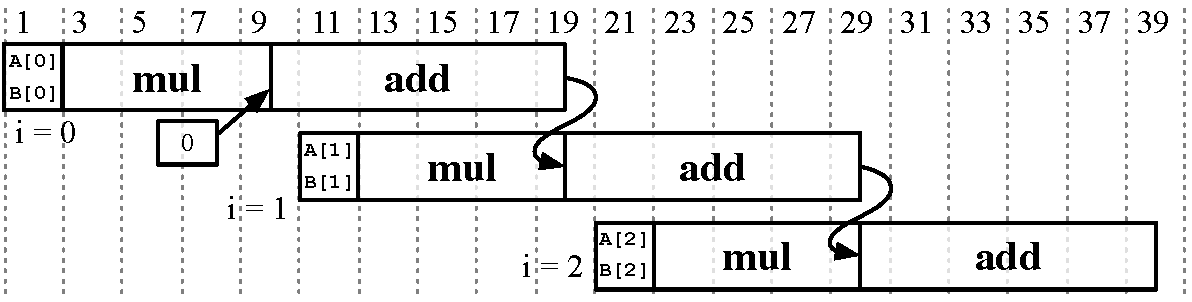
\includegraphics[width=0.8\linewidth]{sample_schedule_before}
    \caption{The resulting schedule of the example program in generated}
    \label{bg:fig:sample_schedule_before}
\end{figure}

Here we see that each iteration requires $18$ cycles, this value is known as
the \emph{depth}, $D$, of the loop.  Because in each iteration, we must wait
for the addition from previous iteration to complete before reading the value
of \verb|d|, \emph{data dependences} exist across iterations.  For this reason,
there are $10$ cycles between the starts of consecutive loop iterations, as
enforced by the data dependences, this value is known as the \emph{initiation
interval}.  Finally, the loop runs for $1024$ iterations (the \emph{trip
count}, $N$), so its overall latency is $((N-1)\times \II) + D = 10250$ cycles.

\begin{figure}[ht]
\begin{lstlisting}
  float d = 0.0f;
  for (int i = 0; i < 1024; i += 2) {
      d = (d + A[i]*B[i]) + A[i+1]*B[i+1];
  }
\end{lstlisting}
    \caption{Partially unrolled version of the original dot-product example.}
    \label{bg:fig:dotprod_unroll}
\end{figure}
Observe that the trip count can be halved by partial unrolling, as shown in
Figure~\ref{bg:fig:dotprod_unroll}.  Since we did not change data-paths by
unrolling, the data dependences remain unchanged, the resulting schedule
and the total latency stay the same.  However, by further exploiting the
associativity of addition, we can delay reading \verb|d| until later in each
iteration (Figure~\ref{bg:fig:dotprod_optimized}).
\begin{figure}[ht]
\begin{lstlisting}
  float d = 0.0f;
  for (int i = 0; i < 1024; i += 2) {
      d = d + (A[i]*B[i] + A[i+1]*B[i+1]);
  }
\end{lstlisting}
    \caption{Partially unrolled code optimized by applying associativity.}
    \label{bg:fig:dotprod_optimized}
\end{figure}

The program now admits the schedule in
Figure~\ref{bg:fig:sample_schedule_after}, which yields a loop latency
of $((512-1)\times 10) + 30 = 5140$ cycles---roughly half the original
latency. This optimized program, which is discovered automatically by our tool,
also reduces round-off errors by 50\% (as a result of the round-off errors
being accumulated in a different order) but increases LUT count by about 35\%
(because more operations are performed in each iteration).

\begin{figure}[ht]
    \centering
    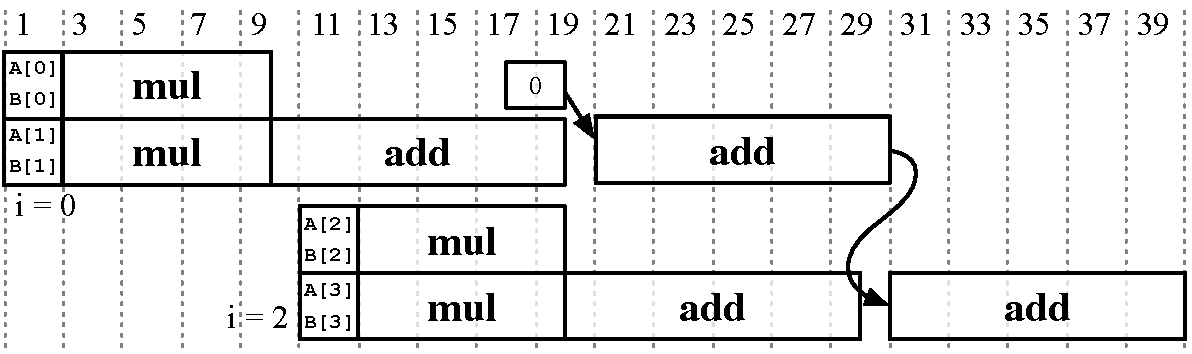
\includegraphics[width=0.8\linewidth]{sample_schedule_after}
    \caption{%
        The resulting schedule of the optimized code in
        Figure~\ref{bg:fig:dotprod_optimized}.}
    \label{bg:fig:sample_schedule_after}
\end{figure}

To accurately analyze the run time of a loop in a numerical program, it is
necessary to generate the schedule of the loop.  Algorithms for this, however,
tend to be computationally expensive, and exacerbated by the fact that we
need to apply this algorithm to each rewritten loops that we have discovered
using transformation rules.  For this we make use of the first few steps of a
scheduling technique known as \emph{iterative modulo scheduling}~\cite{rau94},
to efficiently compute a lower bound on the initiation interval as an
approximation to the actual value, and subsequently, the estimated run time of
the loop.


\subsection{Obstacles in Adoption}
\label{sub:obstacles_in_adoption}


